% Created 2021-01-17 Sun 18:57
% Intended LaTeX compiler: pdflatex
\documentclass[11pt]{article}
\usepackage[utf8]{inputenc}
\usepackage[T1]{fontenc}
\usepackage{graphicx}
\usepackage{grffile}
\usepackage{longtable}
\usepackage{wrapfig}
\usepackage{rotating}
\usepackage[normalem]{ulem}
\usepackage{amsmath}
\usepackage{textcomp}
\usepackage{amssymb}
\usepackage{capt-of}
\usepackage{hyperref}
\usepackage{minted}
\author{Jason Ross}
\date{2021-01-07}
\title{Org Mode \LaTeX{} Demo\\\medskip
\large Baseline Features}
\hypersetup{
 pdfauthor={Jason Ross},
 pdftitle={Org Mode \LaTeX{} Demo},
 pdfkeywords={context org-mode},
 pdfsubject={Comparison of \LaTeX{} to ConTeXt},
 pdfcreator={Jason Ross}, 
 pdflang={English}}
\begin{document}

\maketitle
\tableofcontents


\section{Template Notes}
\label{sec:org4159871}
This is the default \LaTeX{} export with the article class.
\section{Sample Code}
\label{sec:org594f935}
\subsection{{\bfseries\sffamily DONE} \framebox{\#A} Block Elements}
\label{sec:org85b227c}
This section demonstrates different elements delimited by different
\texttt{\#+BEGIN/END} tags.
\index{Source Block}
\subsubsection{Source Blocks}
\label{sec:org1e8c29e}
Syntax highlighting is supported in ConTeXt, but you may have to install a
module to support it. By default, there is a custom ConTeXt \texttt{typing} called
\texttt{OrgBlkSrc} defined in the header that can be customized by adding\\
\texttt{\#+CONTEXT\_HEADER\_EXTRA: \textbackslash{}setuptyping[OrgBlkSrc][...]}.
\begin{minted}[]{python}
import this
for i in range(5):
    print(i * i)
\end{minted}
\index{Verse Block}
\subsubsection{Verse Blocks}
\label{sec:orgd3b33b7}
By default, verse blocks are enclosed in a custom \texttt{\textbackslash{}lines} environment called
\texttt{OrgVerse} that can be customized by adding\\
\texttt{\#+CONTEXT\_HEADER\_EXTRA: \textbackslash{}setuplines[OrgVerse][...]}.

\emph{The Monks and the Giants} by John Hookham Frere
\begin{verse}
But chiefly, when the shadowy moon had shed\\
\hspace*{2em}O'er woods and waters her mysterious hue,\\
Their passive hearts and vacant fancies fed\\
\hspace*{4em}With thoughts and aspirations strange and new,\\
Till their brute souls with inward working bred\\
\hspace*{5em}Dark hints that in the depths of instinct grew\\
Subjection not from Locke's associations,\\
\hspace*{6em}Nor David Hartley's doctrine of vibrations.\\
\end{verse}
\index{Example Block}
\subsubsection{Example Blocks}
\label{sec:orgf78ec1c}
By default, example blocks are enclosed in a custom \texttt{\textbackslash{}typing} environment
called \texttt{OrgExample} that can be customized by adding\\
\texttt{\#+CONTEXT\_HEADER\_EXTRA: \textbackslash{}setuptyping[OrgExample][...]}.

\begin{verbatim}
The Zen of Python, by Tim Peters

Beautiful is better than ugly.
Explicit is better than implicit.
Simple is better than complex.
Complex is better than complicated.
Flat is better than nested.
Sparse is better than dense.
Readability counts.
Special cases aren't special enough to break the rules.
Although practicality beats purity.
Errors should never pass silently.
Unless explicitly silenced.
In the face of ambiguity, refuse the temptation to guess.
There should be one-- and preferably only one --obvious way to do it.
Although that way may not be obvious at first unless you're Dutch.
Now is better than never.
Although never is often better than *right* now.
If the implementation is hard to explain, it's a bad idea.
If the implementation is easy to explain, it may be a good idea.
Namespaces are one honking great idea -- let's do more of those!
\end{verbatim}
\index{Export Block}
\subsubsection{Export Blocks}
\label{sec:orgeefb5cd}
Both \TeX{} and ConTeXt export blocks are supported. Note that you may
have incompatibility issues with \LaTeX{} if your ConTeXt code is labeled
as \TeX{}.
\begin{enumerate}
\item Plain \TeX{}
\label{sec:org381da19}
ABC \quad 123

\item ConTeXt
\label{sec:org69027f0}
\index{Centering}
\end{enumerate}
\subsubsection{Centering}
\label{sec:orgf2426c3}
Centered text just in an \texttt{alignment} environment.

\begin{center}
Nullam eu ante vel est convallis dignissim. Fusce suscipit, wisi nec
facilisis facilisis, est dui fermentum leo, quis tempor ligula erat quis
odio. Nunc porta vulputate tellus. Nunc rutrum turpis sed pede. Sed bibendum.
Aliquam posuere. Nunc aliquet, augue nec adipiscing interdum, lacus tellus
malesuada massa, quis varius mi purus non odio. Pellentesque condimentum,
magna ut suscipit hendrerit, ipsum augue ornare nulla, non luctus diam neque
sit amet urna. Curabitur vulputate vestibulum lorem. Fusce sagittis, libero
non molestie mollis, magna orci ultrices dolor, at vulputate neque nulla
lacinia eros. Sed id ligula quis est convallis tempor. Curabitur lacinia
pulvinar nibh. Nam a sapien.
\end{center}
\index{Quote Block}
\subsubsection{Quote Block}
\label{sec:org3e8c342}
By default, block quotes are enclosed in a custom \texttt{startstop} environment
called \texttt{OrgBlockQuote} that can be customized by adding\\
\texttt{\#+CONTEXT\_HEADER\_EXTRA: \textbackslash{}setupstartstop[OrgBlockQuote][...]}.

\begin{quote}
Aliquam erat volutpat. Nunc eleifend leo vitae magna. In id erat non orci
commodo lobortis. Proin neque massa, cursus ut, gravida ut, lobortis eget,
lacus. Sed diam. Praesent fermentum tempor tellus. Nullam tempus. Mauris ac
felis vel velit tristique imperdiet. Donec at pede. Etiam vel neque nec dui
dignissim bibendum. Vivamus id enim. Phasellus neque orci, porta a, aliquet
quis, semper a, massa. Phasellus purus. Pellentesque tristique imperdiet
tortor. Nam euismod tellus id erat.
\end{quote}
\subsection{Inline Elements}
\label{sec:orgdab7fa0}

\subsubsection{Code}
\label{sec:org77f7c11}
Here's some code: \texttt{with open("file.txt") as f:}

\subsubsection{Links}
\label{sec:org787fb16}
\begin{enumerate}
\item Named URL
\label{sec:orgc7ffdeb}
Here's a link to \href{https://orgmode.org}{Org Mode}
\item Heading Link
\label{sec:orgedb14b5}
Here's a link to \ref{sec:org85b227c}
\item Anonymous url
\label{sec:orgca1b4d7}
Here's a link to \url{https://orgmode.org}
\item Anonymous Unmarked url
\label{sec:org1645fad}
\url{https://orgmode.org}
\end{enumerate}
\subsubsection{Radio Targets}
\label{sec:orgcf380bf}
This is a \label{org188428c}sample radio target

and this is a link to a \hyperref[org188428c]{sample radio target}

\label{orgdb15dd3}
\subsubsection{Target}
\label{sec:org12abfa3}
This is a link to \ref{orgdb15dd3}

TODO

This should refer to the number to match \LaTeX{}
\subsubsection{Bold}
\label{sec:org0f9027e}
This is \textbf{Some bold text}
\subsubsection{\LaTeX{} Fragments}
\label{sec:org636a523}
Here's some inline \LaTeX{}: \(e=m c^2\)
\subsubsection{Inline Source}
\label{sec:orgbf5b4ec}
\texttt{Hello, world!}
\subsubsection{Italic}
\label{sec:org5af85e8}
\emph{This is some italic text}
\subsubsection{Line breaks}
\label{sec:org4540601}
Here is a\\
line break
\subsubsection{Strikethrough}
\label{sec:orgb695a9d}
\sout{This is strikethrough}
\subsubsection{Subscripts}
\label{sec:org14ec1b2}
This\textsubscript{is} sub\textsubscript{script}
\subsubsection{Superscripts}
\label{sec:orge9a6e31}
This\textsuperscript{is} super\textsuperscript{script}
\subsubsection{Underline}
\label{sec:org33c3e07}
\uline{Here's some underlined text}
\subsubsection{Verbatim}
\label{sec:org6e48cee}
\texttt{This is verbatim text}
\subsubsection{Footnote Reference}
\label{sec:org03c8ba9}
Footnotes are formatted with the \texttt{\textbackslash{}footnote} macro. Nested footnotes are
not yet supported.

This should link to a footnote at the bottom of the page. \footnote{This is a sample footnote} 
\subsubsection{Smart Quotes}
\label{sec:orgd403324}
Smart quotes are formatted using the \texttt{\textbackslash{}quote} and \texttt{\textbackslash{}quotation} macros,
which respect language settings.

Here's an English quotation: ``Here's a `nested' quote''

Here's a Czech quotation: ``Here's a `nested' quote''

\subsubsection{Clock}
\label{sec:org6c13ab8}
The default clock is set to use the ISO format. ConTeXt doesn't provide
a locale-aware timestamp but the user can customize the clock appearance
by overriding the \texttt{\textbackslash{}OrgClock} macro. Example: 
\noindent\textbf{CLOCK:} \textit{[2021-01-15 Fri 16:58]}\\


\subsubsection{Timestamp}
\label{sec:org5abf201}
Timestamps are supported by the \texttt{\textbackslash{}date} macro, so different locales
are supported.

Here's an English timestamp: \textit{<2021-01-15 Fri>}

Here's a French timestamp: \textit{<2021-01-15 Fri>}

\subsection{Paragraph Elements}
\label{sec:orgef8222f}
These elements form their own paragraph or section in the export.
\subsubsection{Headlines}
\label{sec:org02697ad}
Headline text is formatted by a custom macro called \texttt{OrgHeadline}
that receives the headline's todo, todo type, priority, text, and
tags. This macro can be overriden by the user to customize the
appearance of headlines.
\subsubsection{\LaTeX{} Environments}
\label{sec:org24ef356}
Common math environments are translated from \LaTeX{} to ConTeXt.

\begin{align*}
\frac{d^4}{dx^4} e^{a x} + e^{a x} &= 0 \\
a^4 e^{a x} + e^{a x} &= 0 \\
a^4 + 1 &= 0 \\
a^4 &= -1 \\
\end{align*}
\subsubsection{Drawer}
\label{sec:orgedca8c4}
This is a simple drawer
\subsubsection{Horizontal Rule}
\label{sec:org7dd17b5}
This is a horizontal rule:

\noindent\rule{\textwidth}{0.5pt}
\subsubsection{Fixed width}
\label{sec:org3793ae5}
Fixed-width text is enclosed in a custom =typing\textasciitilde{} environment
called \texttt{OrgFixed} by default. To customize this environment,\\
add \texttt{\#+CONTEXT\_HEADER\_EXTRA: \textbackslash{}setuptyping[OrgFixed][...]}
to the document.
\begin{verbatim}
This is Some fixed-width text
\end{verbatim}

\subsubsection{Property Drawers}
\label{sec:org6d248b8}
\begin{verbatim}
Title: Goldberg Variations
Composer: J.S. Bach
Artist: Glenn Gould
Publisher: Deutsche Grammophon
NDisks: 1
\end{verbatim}
Property drawers are enclosed in a custom \texttt{typing} environment
called \texttt{OrgPropertyDrawer} by default. To customize this environment,\\
add \texttt{\#+CONTEXT\_HEADER\_EXTRA: \textbackslash{}setuptyping[OrgPropertyDrawer][...]}
to the document.

\subsubsection{Inline Task}
\label{sec:org9bee487}
Inline tasks are supported by a custom \texttt{\textbackslash{}OrgInlineTask} macro.
Arguments to the macro include the todo keyword, the todo type,
the priority, the name of the task, tags, and contents.

Alternatively, for higher-level customization, the user can
provide their own\\
\texttt{org-context-format-inlinetask-function}.



\begin{center}
\fbox{
\begin{minipage}[c]{.6\textwidth}
\textbf{\textsf{\textsc{TODO}}} \framebox{\#B} Check Inline Task\hfill{}\textsc{:tag1:}

\rule[.8em]{\textwidth}{2pt}

\noindent\textbf{DEADLINE:} \textit{<2021-01-22 Fri> } \textbf{SCHEDULED:} \textit{<2021-01-15 Fri>}\\
Lorem ipsum dolor sit amet, consectetuer adipiscing elit. Donec hendrerit tempor
tellus. Donec pretium posuere tellus. Proin quam nisl, tincidunt et, mattis
eget, convallis nec, purus. Cum sociis natoque penatibus et magnis dis
parturient montes, nascetur ridiculus mus. Nulla posuere. Donec vitae dolor.
Nullam tristique diam non turpis. Cras placerat accumsan nulla. Nullam rutrum.
Nam vestibulum accumsan nisl.
\end{minipage}
}
\end{center}

\subsubsection{Lists and items}
\label{sec:orgffd3956}
Standard bulleted lists are enclosed in an \texttt{itemize} environment.
Description lists use a custom \texttt{description} element called
\texttt{OrgDesc}. Additionally, checkbox items use custom macros called
\texttt{OrgItemOn}, \texttt{OrgItemOff}, and \texttt{OrgItemTrans} for the glyphs, so
these can be overriden by the user by adding\\
\texttt{\#+CONTEXT\_HEADER\_EXTRA: \textbackslash{}define\textbackslash{}OrgItemOn\{...\}}
to the document.

\begin{itemize}
\item Bullet 1
\item Bullet 2
\item Bullet 3
\begin{itemize}
\item SubBullet 1
\item[{$\boxminus$}] SubBullet 2 [1/2]
\begin{itemize}
\item[{$\boxtimes$}] SubSubBullet 1
\item[{$\square$}] SubSubBullet 2
\end{itemize}
\end{itemize}
\end{itemize}


\begin{description}
\item[{Description Item 1}] Nullam eu ante vel est convallis dignissim. Fusce
suscipit, wisi nec facilisis facilisis, est dui fermentum leo, quis tempor
ligula erat quis odio. Nunc porta vulputate tellus. Nunc rutrum turpis sed
pede. Sed bibendum. Aliquam posuere. Nunc aliquet, augue nec adipiscing
interdum, lacus tellus malesuada massa, quis varius mi purus non odio.
Pellentesque condimentum, magna ut suscipit hendrerit, ipsum augue ornare
nulla, non luctus diam neque sit amet urna. Curabitur vulputate vestibulum
lorem. Fusce sagittis, libero non molestie mollis, magna orci ultrices
dolor, at vulputate neque nulla lacinia eros. Sed id ligula quis est
convallis tempor. Curabitur lacinia pulvinar nibh. Nam a sapien.
\item[{$\boxtimes$ Description Item 2}] Checked
\item[{$\square$ Description Item 3}] Unchecked
\item[{$\boxminus$ Description Item 4 [1/2]}] Transatory
\begin{itemize}
\item[{$\square$}] Sub1
\item[{$\boxtimes$}] Sub2
\end{itemize}
\end{description}


\begin{enumerate}
\item Numbered item
\item Another Number
\end{enumerate}

\subsubsection{Tables}
\label{sec:orgaa8bb75}
Tables are supported by the \texttt{xtables} environment.

\begin{table}[htbp]
\caption{Default Layout Table}
\centering
\begin{tabular}{rr}
A & B\\
\hline
1 & 2\\
3 & 4\\
\end{tabular}
\end{table}

Here's the same table with \texttt{:option width}

\begin{table}[htbp]
\caption{Wide Layout Table}
\centering
\begin{tabular}{rr}
A & B\\
\hline
1 & 2\\
3 & 4\\
\end{tabular}
\end{table}

Here's the same table with \texttt{:option tight}

\begin{table}[htbp]
\caption{Tight Layout Table}
\centering
\begin{tabular}{rr}
A & B\\
\hline
1 & 2\\
3 & 4\\
\end{tabular}
\end{table}


Here's the same table with \texttt{:option stretch}

\begin{table}[htbp]
\caption{Stretch Layout Table}
\centering
\begin{tabular}{rr}
A & B\\
\hline
1 & 2\\
3 & 4\\
\end{tabular}
\end{table}


Here's a very long table. We can split it by setting
\texttt{:split t} and \texttt{:header repeat} in \texttt{\#+ATTR\_CONTEXT}.

\begin{table}[htbp]
\caption{Giant Table}
\centering
\begin{tabular}{rrrrrrrrrr}
A & B & C & D & E & F & G & H & I & J\\
\hline
0 & 0 & 0 & 0 & 0 & 0 & 0 & 0 & 0 & 0\\
0 & 1 & 2 & 3 & 4 & 5 & 6 & 7 & 8 & 9\\
0 & 2 & 4 & 6 & 8 & 10 & 12 & 14 & 16 & 18\\
0 & 3 & 6 & 9 & 12 & 15 & 18 & 21 & 24 & 27\\
0 & 4 & 8 & 12 & 16 & 20 & 24 & 28 & 32 & 36\\
0 & 5 & 10 & 15 & 20 & 25 & 30 & 35 & 40 & 45\\
0 & 6 & 12 & 18 & 24 & 30 & 36 & 42 & 48 & 54\\
0 & 7 & 14 & 21 & 28 & 35 & 42 & 49 & 56 & 63\\
0 & 8 & 16 & 24 & 32 & 40 & 48 & 56 & 64 & 72\\
0 & 9 & 18 & 27 & 36 & 45 & 54 & 63 & 72 & 81\\
0 & 10 & 20 & 30 & 40 & 50 & 60 & 70 & 80 & 90\\
0 & 11 & 22 & 33 & 44 & 55 & 66 & 77 & 88 & 99\\
0 & 12 & 24 & 36 & 48 & 60 & 72 & 84 & 96 & 108\\
0 & 13 & 26 & 39 & 52 & 65 & 78 & 91 & 104 & 117\\
0 & 14 & 28 & 42 & 56 & 70 & 84 & 98 & 112 & 126\\
0 & 15 & 30 & 45 & 60 & 75 & 90 & 105 & 120 & 135\\
0 & 16 & 32 & 48 & 64 & 80 & 96 & 112 & 128 & 144\\
0 & 17 & 34 & 51 & 68 & 85 & 102 & 119 & 136 & 153\\
0 & 18 & 36 & 54 & 72 & 90 & 108 & 126 & 144 & 162\\
0 & 19 & 38 & 57 & 76 & 95 & 114 & 133 & 152 & 171\\
0 & 20 & 40 & 60 & 80 & 100 & 120 & 140 & 160 & 180\\
0 & 21 & 42 & 63 & 84 & 105 & 126 & 147 & 168 & 189\\
0 & 22 & 44 & 66 & 88 & 110 & 132 & 154 & 176 & 198\\
0 & 23 & 46 & 69 & 92 & 115 & 138 & 161 & 184 & 207\\
0 & 24 & 48 & 72 & 96 & 120 & 144 & 168 & 192 & 216\\
0 & 25 & 50 & 75 & 100 & 125 & 150 & 175 & 200 & 225\\
0 & 26 & 52 & 78 & 104 & 130 & 156 & 182 & 208 & 234\\
0 & 27 & 54 & 81 & 108 & 135 & 162 & 189 & 216 & 243\\
0 & 28 & 56 & 84 & 112 & 140 & 168 & 196 & 224 & 252\\
0 & 29 & 58 & 87 & 116 & 145 & 174 & 203 & 232 & 261\\
0 & 30 & 60 & 90 & 120 & 150 & 180 & 210 & 240 & 270\\
0 & 31 & 62 & 93 & 124 & 155 & 186 & 217 & 248 & 279\\
0 & 32 & 64 & 96 & 128 & 160 & 192 & 224 & 256 & 288\\
0 & 33 & 66 & 99 & 132 & 165 & 198 & 231 & 264 & 297\\
0 & 34 & 68 & 102 & 136 & 170 & 204 & 238 & 272 & 306\\
0 & 35 & 70 & 105 & 140 & 175 & 210 & 245 & 280 & 315\\
0 & 36 & 72 & 108 & 144 & 180 & 216 & 252 & 288 & 324\\
0 & 37 & 74 & 111 & 148 & 185 & 222 & 259 & 296 & 333\\
0 & 38 & 76 & 114 & 152 & 190 & 228 & 266 & 304 & 342\\
0 & 39 & 78 & 117 & 156 & 195 & 234 & 273 & 312 & 351\\
0 & 40 & 80 & 120 & 160 & 200 & 240 & 280 & 320 & 360\\
0 & 41 & 82 & 123 & 164 & 205 & 246 & 287 & 328 & 369\\
0 & 42 & 84 & 126 & 168 & 210 & 252 & 294 & 336 & 378\\
0 & 43 & 86 & 129 & 172 & 215 & 258 & 301 & 344 & 387\\
0 & 44 & 88 & 132 & 176 & 220 & 264 & 308 & 352 & 396\\
0 & 45 & 90 & 135 & 180 & 225 & 270 & 315 & 360 & 405\\
0 & 46 & 92 & 138 & 184 & 230 & 276 & 322 & 368 & 414\\
0 & 47 & 94 & 141 & 188 & 235 & 282 & 329 & 376 & 423\\
0 & 48 & 96 & 144 & 192 & 240 & 288 & 336 & 384 & 432\\
0 & 49 & 98 & 147 & 196 & 245 & 294 & 343 & 392 & 441\\
\end{tabular}
\end{table}

Here's a table with paragraphs in it. ConTeXt handles this gracefully by
default.

\begin{table}[htbp]
\caption{Wrapped Table}
\centering
\begin{tabular}{ll}
Description & Contents\\
\hline
First Thing & Aliquam erat volutpat.  Nunc eleifend leo vitae magna.  In id erat non orci commodo lobortis.  Proin neque massa, cursus ut, gravida ut, lobortis eget, lacus.  Sed diam.  Praesent fermentum tempor tellus.  Nullam tempus.  Mauris ac felis vel velit tristique imperdiet.  Donec at pede.  Etiam vel neque nec dui dignissim bibendum.  Vivamus id enim.  Phasellus neque orci, porta a, aliquet quis, semper a, massa.  Phasellus purus.  Pellentesque tristique imperdiet tortor.  Nam euismod tellus id erat.\\
Second Thing & Pellentesque dapibus suscipit ligula.  Donec posuere augue in quam.  Etiam vel tortor sodales tellus ultricies commodo.  Suspendisse potenti.  Aenean in sem ac leo mollis blandit.  Donec neque quam, dignissim in, mollis nec, sagittis eu, wisi.  Phasellus lacus.  Etiam laoreet quam sed arcu.  Phasellus at dui in ligula mollis ultricies.  Integer placerat tristique nisl.  Praesent augue.  Fusce commodo.  Vestibulum convallis, lorem a tempus semper, dui dui euismod elit, vitae placerat urna tortor vitae lacus.  Nullam libero mauris, consequat quis, varius et, dictum id, arcu.  Mauris mollis tincidunt felis.  Aliquam feugiat tellus ut neque.  Nulla facilisis, risus a rhoncus fermentum, tellus tellus lacinia purus, et dictum nunc justo sit amet elit.\\
\end{tabular}
\end{table}

Here's a shorter table.

\begin{table}[htbp]
\caption{Short Table}
\centering
\begin{tabular}{rrrrrrrrrr}
A & B & C & D & E & F & G & H & I & J\\
\hline
0 & 0 & 0 & 0 & 0 & 0 & 0 & 0 & 0 & 0\\
0 & 1 & 2 & 3 & 4 & 5 & 6 & 7 & 8 & 9\\
0 & 2 & 4 & 6 & 8 & 10 & 12 & 14 & 16 & 18\\
0 & 3 & 6 & 9 & 12 & 15 & 18 & 21 & 24 & 27\\
0 & 4 & 8 & 12 & 16 & 20 & 24 & 28 & 32 & 36\\
0 & 5 & 10 & 15 & 20 & 25 & 30 & 35 & 40 & 45\\
0 & 6 & 12 & 18 & 24 & 30 & 36 & 42 & 48 & 54\\
0 & 7 & 14 & 21 & 28 & 35 & 42 & 49 & 56 & 63\\
\end{tabular}
\end{table}

TODO: Allow table-style to take keyword arguments

Tables can be customized in several ways. By default, the top and bottom rows,
the left and right columns, and the four corners of the table have special
styles which default to \texttt{OrgTableTopRow}, \texttt{OrgTableBottomRow},
\texttt{OrgTableLeftCol}, \texttt{OrgTableRightCol}, \texttt{OrgTableTopLeftCell},
\texttt{OrgTableTopRightCell}, \texttt{OrgTableBottomRightCell}, and
\texttt{OrgTableBottomLeftCell}. These styles can be configured by adding\\
\texttt{\#+CONTEXT\_HEADER\_EXTRA: \textbackslash{}setupxtable[OrgTable...][...]} to the document.
Styling options for individual tables can be configured using the
\texttt{:top}, \texttt{:bottom}, \texttt{:left}, \texttt{:right}, \texttt{:topleft}, \texttt{:topright}, \texttt{:bottomright}
and \texttt{:bottomleft} keywords in \texttt{\#+ATTR\_CONTEXT}.
\begin{table}[htbp]
\caption{Fancy Table}
\centering
\begin{tabular}{rrrr}
A & B & C & D\\
\hline
0 & 0 & 0 & 0\\
0 & 1 & 2 & 3\\
0 & 2 & 4 & 6\\
\end{tabular}
\end{table}


\subsubsection{Other Features}
\label{sec:org594022a}
\begin{enumerate}
\item Levels
\label{sec:org347b698}
Many levels of subheading are supported by ConTeXt (up to 9). If more levels
are needed, the user can create them using the \texttt{\textbackslash{}definehead} macro. To handle
10 levels, for example, add \\
\texttt{\#+CONTEXT\_HEADER\_EXTRA: \textbackslash{}definehead[subsubsubsubsubsubsubsubsubsection]
    [subsubsubsubsubsubsubsubsection]} \\
to the document.
\begin{quote}
The \LaTeX{} exporter handles arbitrarily deep nesting by treating deeper
headings as list elements, but true headlines are only supported down
to 5 levels deep.
\end{quote}
\begin{enumerate}
\item Level 4
\label{sec:orgb8f5136}
\begin{enumerate}
\item Level 5
\label{sec:org1d8a34e}
\begin{enumerate}
\item Level 6
\label{sec:orgf1e3481}
\begin{enumerate}
\item Level 7
\label{sec:org289de1e}
\begin{enumerate}
\item Level 8
\label{sec:org9606cb1}
\begin{enumerate}
\item Level 9
\label{sec:org5c5163f}
\end{enumerate}
\end{enumerate}
\end{enumerate}
\end{enumerate}
\end{enumerate}
\end{enumerate}
\item Images
\label{sec:orgab4ff1d}
Inline images are supported.

\begin{minted}[]{org}
#+CAPTION: Default Figure
[[./bessel11.pdf]]
\end{minted}

\begin{figure}[htbp]
\centering
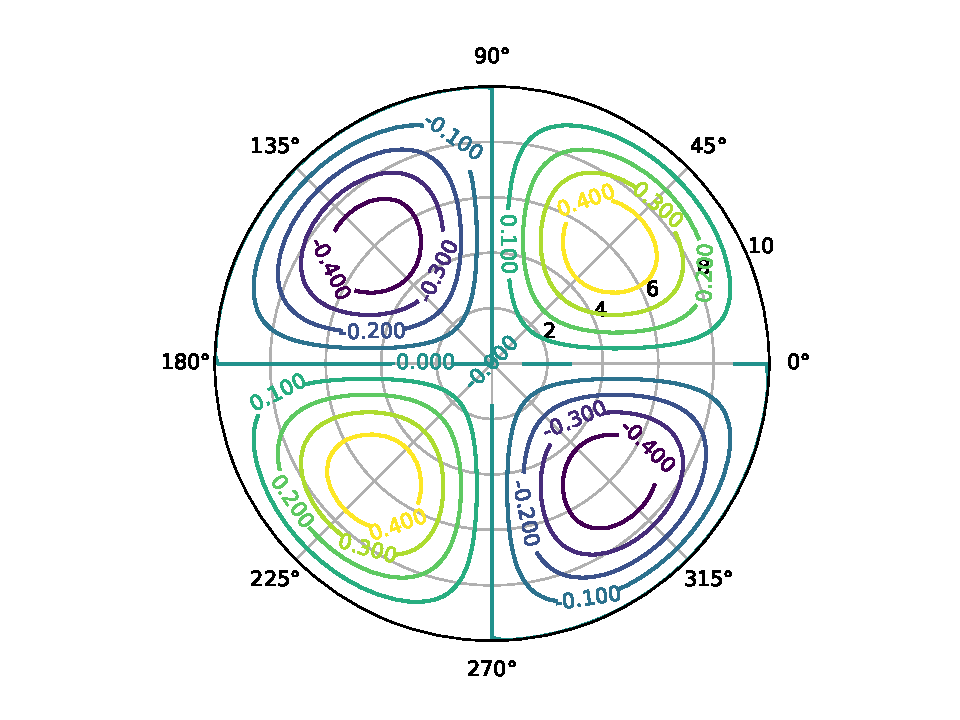
\includegraphics[width=.9\linewidth]{./bessel11.pdf}
\caption{Default Figure}
\end{figure}

Nullam eu ante vel est convallis dignissim. Fusce suscipit, wisi nec facilisis
facilisis, est dui fermentum leo, quis tempor ligula erat quis odio. Nunc porta
vulputate tellus. Nunc rutrum turpis sed pede. Sed bibendum. Aliquam posuere.
Nunc aliquet, augue nec adipiscing interdum, lacus tellus malesuada massa, quis
varius mi purus non odio. Pellentesque condimentum, magna ut suscipit hendrerit,
ipsum augue ornare nulla, non luctus diam neque sit amet urna. Curabitur
vulputate vestibulum lorem. Fusce sagittis, libero non molestie mollis, magna
orci ultrices dolor, at vulputate neque nulla lacinia eros. Sed id ligula quis
est convallis tempor. Curabitur lacinia pulvinar nibh. Nam a sapien.

\begin{minted}[]{org}
#+ATTR_CONTEXT: :float wrap :caption Default Wrapped Figure
[[./bessel11.pdf]]
\end{minted}

\begin{wrapfigure}{l}{0.5\textwidth}
\centering
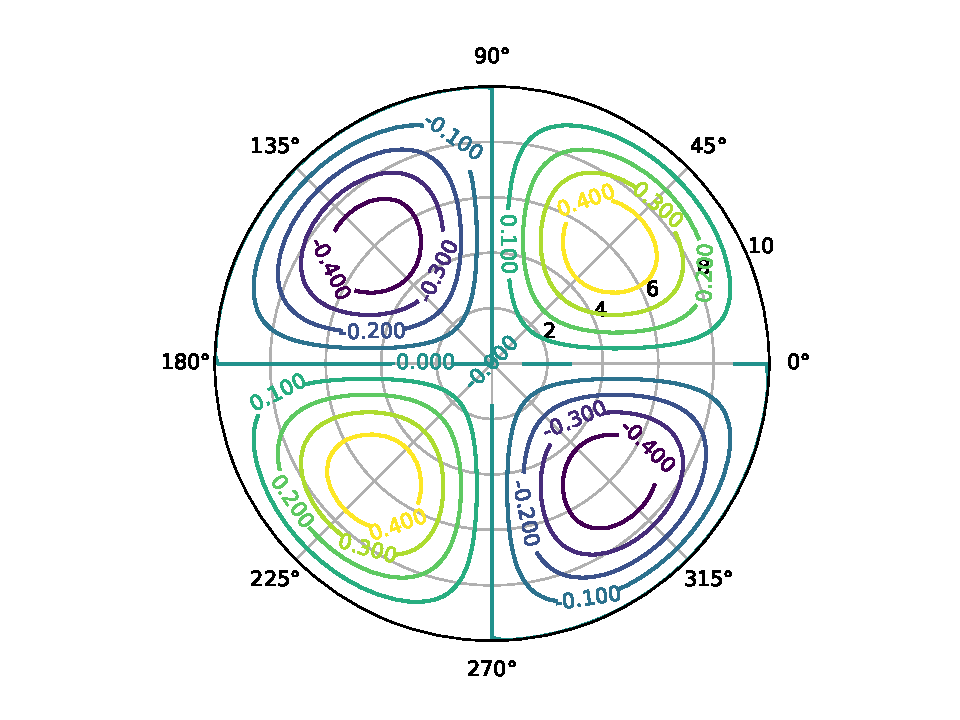
\includegraphics[width=0.48\textwidth]{./bessel11.pdf}
Default Wrapped Figure
\end{wrapfigure}

Nullam eu ante vel est convallis dignissim. Fusce suscipit, wisi nec facilisis
facilisis, est dui fermentum leo, quis tempor ligula erat quis odio. Nunc
porta vulputate tellus. Nunc rutrum turpis sed pede. Sed bibendum. Aliquam
posuere. Nunc aliquet, augue nec adipiscing interdum, lacus tellus malesuada
massa, quis varius mi purus non odio. Pellentesque condimentum, magna ut
suscipit hendrerit, ipsum augue ornare nulla, non luctus diam neque sit amet
urna. Curabitur vulputate vestibulum lorem. Fusce sagittis, libero non
molestie mollis, magna orci ultrices dolor, at vulputate neque nulla lacinia
eros. Sed id ligula quis est convallis tempor. Curabitur lacinia pulvinar
nibh. Nam a sapien.

Aliquam erat volutpat. Nunc eleifend leo vitae magna. In id erat non orci
commodo lobortis. Proin neque massa, cursus ut, gravida ut, lobortis eget,
lacus. Sed diam. Praesent fermentum tempor tellus. Nullam tempus. Mauris ac
felis vel velit tristique imperdiet. Donec at pede. Etiam vel neque nec dui
dignissim bibendum. Vivamus id enim. Phasellus neque orci, porta a, aliquet
quis, semper a, massa. Phasellus purus. Pellentesque tristique imperdiet
tortor. Nam euismod tellus id erat.

Nullam eu ante vel est convallis dignissim. Fusce suscipit, wisi nec facilisis
facilisis, est dui fermentum leo, quis tempor ligula erat quis odio. Nunc
porta vulputate tellus. Nunc rutrum turpis sed pede. Sed bibendum. Aliquam
posuere. Nunc aliquet, augue nec adipiscing interdum, lacus tellus malesuada
massa, quis varius mi purus non odio. Pellentesque condimentum, magna ut
suscipit hendrerit, ipsum augue ornare nulla, non luctus diam neque sit amet
urna. Curabitur vulputate vestibulum lorem. Fusce sagittis, libero non
molestie mollis, magna orci ultrices dolor, at vulputate neque nulla lacinia
eros. Sed id ligula quis est convallis tempor. Curabitur lacinia pulvinar
nibh. Nam a sapien.


Lorem ipsum dolor sit amet, consectetuer adipiscing elit. Donec hendrerit
tempor tellus. Donec pretium posuere tellus. Proin quam nisl, tincidunt et,
mattis eget, convallis nec, purus. Cum sociis natoque penatibus et magnis dis
parturient montes, nascetur ridiculus mus. Nulla posuere. Donec vitae dolor.
Nullam tristique diam non turpis. Cras placerat accumsan nulla. Nullam rutrum.
Nam vestibulum accumsan nisl.

\begin{minted}[]{org}
#+ATTR_CONTEXT: :width 1in :placement rightmargin 
#+CAPTION: Margin Figure
[[./bessel11.pdf]]
\end{minted}

\begin{figure}right
\centering
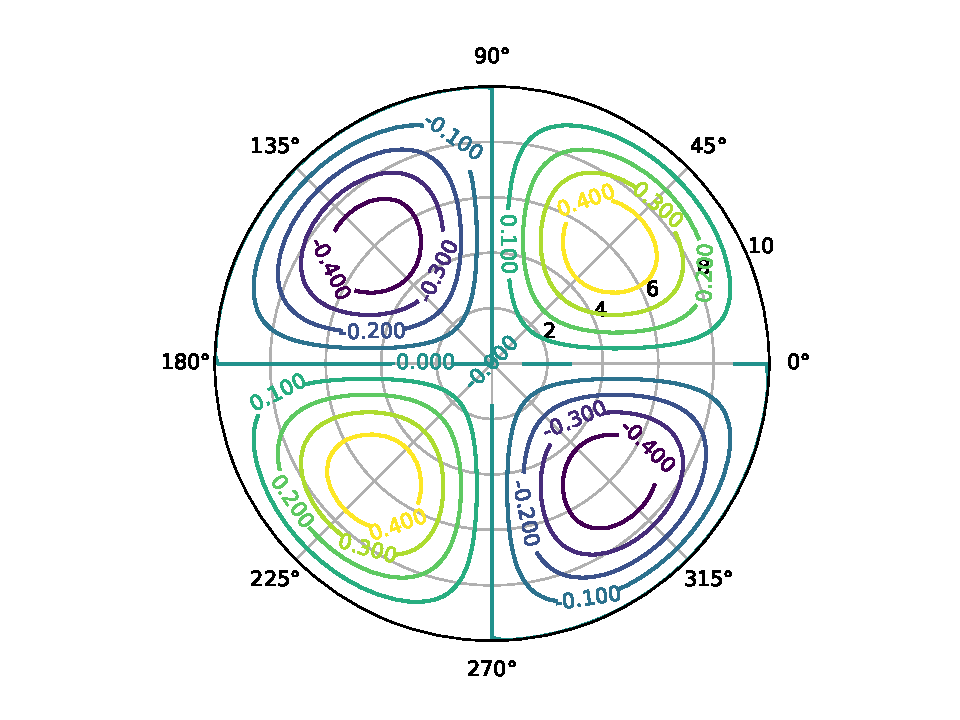
\includegraphics[width=1in]{./bessel11.pdf}
\caption{Margin Figure}
\end{figure}

Aliquam erat volutpat. Nunc eleifend leo vitae magna. In id erat non orci
commodo lobortis. Proin neque massa, cursus ut, gravida ut, lobortis eget,
lacus. Sed diam. Praesent fermentum tempor tellus. Nullam tempus. Mauris ac
felis vel velit tristique imperdiet. Donec at pede. Etiam vel neque nec dui
dignissim bibendum. Vivamus id enim. Phasellus neque orci, porta a, aliquet
quis, semper a, massa. Phasellus purus. Pellentesque tristique imperdiet
tortor. Nam euismod tellus id erat.

Aliquam erat volutpat. Nunc eleifend leo vitae magna. In id erat non orci
commodo lobortis. Proin neque massa, cursus ut, gravida ut, lobortis eget,
lacus. Sed diam. Praesent fermentum tempor tellus. Nullam tempus. Mauris ac
felis vel velit tristique imperdiet. Donec at pede. Etiam vel neque nec dui
dignissim bibendum. Vivamus id enim. Phasellus neque orci, porta a, aliquet
quis, semper a, massa. Phasellus purus. Pellentesque tristique imperdiet tortor.
Nam euismod tellus id erat.
\end{enumerate}

\subsection{Index}
\label{sec:orge2757c8}
We can place an index in the document using \texttt{\#+CONTEXT: \textbackslash{}placeindex}
\end{document}